
\addcontentsline{toc}{subsubsection}{Illustrations: Modulus}
\vbtitle{\textbf{Illustrations: Modulus}}
\BgThispage
\begin{enumerate}
    \item $|x-1|=1$
        \begin{solution}
            \begin{multicols}{2}
            \begin{align*}
                \intertext{By breaking modulus:}
                |x-1| &= 1\\
                |x-1| &= \begin{cases}
                    x-1 & \text{if } x-1 \geq 0\\
                    -(x-1) & \text{if } x-1 < 0
                \end{cases}\\
                &= \begin{cases}
                    x-1 & \text{if } x \geq 1\\
                    -(x-1) & \text{if } x < 1
                \end{cases}\\
                \intertext{For \( x \geq 1 \):}
                x-1 &= 1\\
                x &= 2\\
                \intertext{For \( x < 1 \):}
                -(x-1) &= 1\\
                x-1 &= -1\\
                x &= 0\\
                \Aboxed{x &= 0, 2}
                \end{align*}
                \begin{align*}
                \intertext{Alternatively,}
                \intertext{Squaring both sides:}
                (x-1)^2 &= 1\\
                x^2-2x+1 &= 1\\
                x^2-2x &= 0\\
                x(x-2) &= 0\\
                \Aboxed{x &= 0, 2}
                \intertext{Squaring produces extraneous roots. So you must check the roots.}
            \end{align*}
            \begin{center}
                \begin{tikzpicture}
                    \tzaxes(-2, -0.5)(4, 2){$x$}{$y$}
                    \tzfn{1}[-1:3]{$y=1$}[r]
                    \tzfn{\x-1}[1:3]{$|x-1|$}[r]
                    \tzfn{-\x+1}[-1:1]
                    \tzdot*(0, 1)
                    \tzdot*(2, 1)
                    \tzline[dashed](2, 0)(2, 1)
                    \tzticks{1, 2}
                    \tznode(0, 3){\text{Alternatively, graphically:}}
                \end{tikzpicture}
            \end{center}
            \end{multicols}
        \end{solution}

    \item $|x-1| = |x+1|$
        \begin{solution}
            \begin{multicols}{2}
                \vspace*{-13mm}
            \begin{align*}
                \intertext{By breaking modulus: If there are more than one factor in the modulus, then the best way is to break into intervals. For that you need zero every factor and find out the critical points and plot them on the number line.}
                x-1 = 0 \quad &\text{and} \quad x+1 = 0\\
                x = 1 \quad &\text{and} \quad x = -1\\
            \end{align*}
                \begin{center}
                    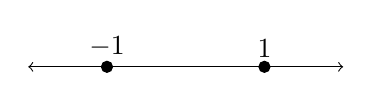
\begin{tikzpicture}
                        \draw[<->](-2, 0)--(2, 0);
                        \draw[fill=black](1, 0) circle (2pt) node[above]{$1$};
                        \draw[fill=black](-1, 0) circle (2pt) node[above]{$-1$};
                    \end{tikzpicture}
                \end{center}
            \begin{align*}
                \intertext{Now, number line is divided into three intervals:}
                \intertext{For \( x < -1 \):}
                -(x-1) &= -(x+1)\\
                -x+1 &= -x-1\\
                1 &= -1\\
                \intertext{No solution.}
                \intertext{For \( -1 \leq x \leq 1 \):}
                -(x-1) &= x+1\\
                -x+1 &= x+1\\
                2x &=0\\
                x &= 0\\
                \intertext{We got a solution, but we have to check it, is it in the interval or not. In this case, it is in the interval. So the solution is \( x = 0 \).}
                \intertext{For \( x > 1 \):}
                x-1 &= x+1\\
                -1 &= 1\\
                \intertext{No solution.}
            \end{align*}
            
            \begin{align*}
                \intertext{Alternatively,}
                \intertext{Squaring both sides:}
                (x-1)^2 &= (x+1)^2\\
                x^2-2x+1 &= x^2+2x+1\\
                -2x &= 2x\\
                \Aboxed{x &= 0}
                \intertext{Squaring produces extraneous roots. So you must check the roots.}
            \end{align*}
            % \begin{center}
            %     \begin{tikzpicture}
            %         \tzaxes(-2, -0.5)(2, 2){$x$}{$y$}
            %         \tzfn{\x-1}[-1:2]{$|x-1|$}[r]
            %         \tzfn{-\x-1}[-2:1]{$|x+1|$}[r]
            %         \tzdot*(0, 1)
            %         \tzline[dashed](0, 0)(0, 1)
            %         \tzticks{-1, 1}
            %         \tznode(0, 3){\text{Alternatively, graphically:}}
            %     \end{tikzpicture}
            % \end{center}
            \end{multicols}
        \end{solution}
        \BgThispage
    \item $|x^2 -x -6| = x+2$
        \begin{solution}
            \begin{align*}
                \intertext{Equate factors of the modulus to zero:}
                x^2-x-6 &= 0\\
                x^2-3x+2x-6 &= 0\\
                x(x-3)+2(x-3) &= 0\\
                (x+2)(x-3) &= 0\\
                x &= -2, 3
            \end{align*}
            \begin{center}
                \begin{tikzpicture}
                    \draw[<->](-3, 0)--(4, 0);
                    \draw[fill=black](-1, 0) circle (2pt) node[above]{$-2$};
                    \draw[fill=black](2, 0) circle (2pt) node[above]{$3$};
                \end{tikzpicture}
            \end{center}
            \begin{align*}
                \intertext{Now, number line is divided into three intervals:}
                \intertext{For \( x \leq -2 \):}
                \intertext{Put any number within the interval in the equation and check the sign of the equation.}
                \intertext{Let's put \( x = -3 \): \( x^2-x-6 = 9+3-6 = 6 \), +ve. Modulus will do nothing.}
                x^2-x-6 &= x+2\\
                x^2-2x-8 &= 0\\
                (x-4)(x+2) &= 0\\
                x &= -2, 4
                \intertext{We got two solution but only one is in the interval. So the solution is \( x = -2 \).}
                \intertext{For \( -2 < x < 3 \):}
                -(x^2-x-6) &= x+2\\
                -x^2+x+6 &= x+2\\
                -x^2 + 4 &= 0\\
                x^2 &= 4\\
                x &= \pm 2
                \intertext{We got two solution but only one is in the interval. So the solution is \( x = 2 \).}
                \intertext{For \( x \geq 3 \):}
                x^2-x-6 &= x+2\\
                x^2-2x-8 &= 0\\
                (x-4)(x+2) &= 0\\
                x &= -2, 4
                \intertext{We got two solution but only one is in the interval. So the solution is \( x = 4 \).}
                \Aboxed{x &= -2, 2, 4}
            \end{align*}
            \vbstarednote{We could have solved both positive intervals at once for \( x \leq -2 \) and \(x\geq 3\).}
        \end{solution}
\end{enumerate}